\section{Introduction}\label{sec::introduction}
\subsection{Motivation}
% Overall context
Ever growing amounts of data require effective and efficient storage solutions as well as scalable, interactive methods to gain new insights through exploratory analysis or to prove assumptions. Almost all data is subject to change. Nowadays storage is cheap and adheres to Moore's law\cite{MOORE} of doubling about every 18 months, thus supporting the storage of several snapshots of time varying data. Furthermore existing storage solutions minimize the impact of storing such potentially very large data-sets.

Hierarichal information in the form of tree-structures is inherent to many datasets. It is almost always mapped through primary-/foreign-key relations in relational databases. Whereas this might be sufficient in many situations it introduces an additional artificial mapping. Instead, using either a graph-DBMS for directed acyclic graphs (DAGs) or a native XML-DBMS for tree-structures facilitates a straight forward approach of storing data as well as efficient traversal methods and other domain specific advantages (for instance Dijkstra's algorithm for shortest path search in graph databases and most often extensive XQuery support in XML-DBMS).

\subsubsection{Comparison of tree-structures}
In order to be human readable every tree-structure has to be serializable in some form. Utilizing state-of-the-art character based line by line comparsion difference-tools as for instance used within Subversion (SVN\cite{SUBVERSION}) or the GNU diff tool to compare serialized textual tree-structure representations most often does not add up. Even though most of them color-encode the character-based differences or provide other limited graphical representations of the computed differences they are not able to recognize the tree-structure and certain domain specific characteristics. For instance XML (Extensible Markup Language), which is a human readable meta markup language, exemplary for tree-structures in general and used in our prototype, has some inherent features which can not be recognized by such tools. Among those are the \emph{lack of semantic differences} in case two XML documents only differ by an arbitrary amount of whitespace between attributes, namespaces\footnote{special kind of attributes} and elements or the permutation of attributes. Changes from empty elements to start tag, end tag sequences (\texttt{<root/>} to \texttt{<root></root>}) or inversely must not be recognized as a semantic difference as well. The major disadvantage however attributes to the tree-structure itself. Node-boundaries can not be recognized as these tools incorporate no knowledge about the structure itself. Furthermore moves of nodes or subtrees and differences in the order of child nodes can not be detected. A comparison between two very simple XML documents (or two versions thereof) with GVim, which utilizes a line by line character based comparison algorithm is illustrated in Fig. \ref{fig:faileddiff}. Several of the aforementioned deficiencies are depicted in this simple example. 

\begin{figure}[tb]
\center{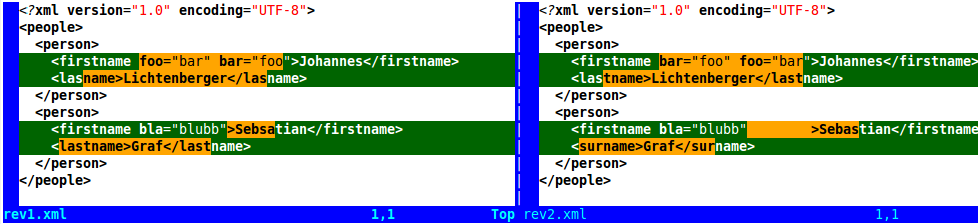
\includegraphics[width=\textwidth]
{figures/gvimdiff.png}}
\caption{\label{fig:faileddiff} GVim diff of two XML-document revisions illustrating the deficiencies of line by line character based diff-tools.}
\end{figure}

\subsection{Problem Statement}\label{subsec::problem}
% Problem statement
%Todays challenges in database research includes the analysis of increasingly large amounts of data. Storing not only one version of a tree-structure but several similar versions proves this task. Analysts typically face the problem of quickly gaining knowledge from a database with potentially large amounts of uninteresting data for the task at hand. They literally have to find a needle in a haystack, which is commonly known as the "information overload" problem. 
Analysts often face the problem of having to compare large tree-structures. While coping with rapidly increasing amounts of data is effectively solved by means of Treetank, a tree-storage system used by our prototype, comparison requires sophisticated methods on top of it. 

Generally two cases of tree-structures have to be distinguished which our system must be capable of.

\begin{itemize}
\item Tree-structures evolving naturally through applying changes.
\item Similar tree-structures.
\end{itemize}

The research task adressed in this thesis is the problem of how to support analyts in comparing tree-structures.

\subsection{Approach}
% Approach
A promising solution to the task at hand is to use methods from "Visual Analytics", a term coined by James J. Thomas in \cite{VISUAL_ANALYTICS}. Thomas states that Visual Analytics is "the science of analytical reasoning facilitated by visual interactive interfaces". Thus we provide analytical methods which are inevitable for comparing tree-structures in the first place facilitated by an interactive visual interface. Furthermore interesting patterns can be revealed by custom \texttt{XPath} queries.

Whereas hierarichal visualizations have been studied for some time and sophisticated representations have been found, Visual Analytics of comparing tree-structures just recently gained momentum.

\subsubsection{Value of visualizations}
Francis J. Anscombe reveals the value of graphs (which is generalizable to every (useful) kind of data-visualization) by illustrating in a simple example with four data sets (Anscombe's quartet), why graphs are essential to good (statistical) analysis. Using statistical calculations from a typical regression program (mean, variance, correlation and linear regression) shows that each computation yields almost the same result even though fundamental differences are visible on first glance once plotted. Furthermore Human brains are trained to interpret visual- instead of textual-content. It is almost impossible to gain further insights running through the printed out form of these four datasets \cite{ANSCOMBE}. 

\subsubsection{Generalization and refinement of our research task}
While several data mining tools are available which specify on specific tasks, tree-structures are flexible and come in many shapes. XML is a semi-structured meta markup language which is capable of describing all kinds of rooted, labeled trees. Thus it is used by our prototype. XML-documents in stark contrast to relational data do not have to adhere to a schema, which has to be planned and implemented beforehand. Due to that it is mandatory that the visual interface offers great flexibility and thus is not restricted to a special use case.

The high level goal defined in section (\ref{subsec::problem}) can be divided into:

\begin{itemize}
\item Preprocessing and import of differences without having to rely on unique node identifiers.
\item Structural comparison based on \texttt{insert-/delete-}operations.
\item Comparison of non-structural data (for instance \texttt{TextNode} values).
\item Extend with \texttt{replace}, \texttt{update} and \texttt{move}-operations (optional).
\item Provide visualizations to quickly gain insights into which subtrees/nodes have been changed.
\end{itemize}

\subsection{Contributions}
The main aim of this thesis is the research and development of an interactive visual interface supporting analysts in comparing tree-structures along with analytical methods to compute the differences in the first place.

In a nutshell this thesis provides the following computer science contributions:

\begin{itemize}
\item Preprocessing of realworld XML data, for instance the revisioned import of (a small fraction of) \emph{Wikipedia} and monitoring changes in a specific Filesystem directory.
\item Several storage-enhancements of a database-system tailored to the storage of temporal tree-structures including compacting, a LevelOrderAxis and new edit-operations to support the implementation of an ID-based differencing algorithm as well as expressive visualizations. Furthermore a new bulk-insertion operation based on an existing component speeds up hashing of subtrees considerably from $O(n^2+m)$ to $O(n+m)$ due to a simple postprocessing postorder traversal whereas $n$ is the size of the nodes in the inserted subtree and $m$ the number of ancestor nodes of the inserted node/subtree.
\item Analytical methods (algorithms) to compute structural and non structural differences between similar or evolving tree-structures.
\item Several views:
\begin{itemize}
\item A \texttt{TextView} which serializes an aggregated tree-structure to a syntax highlighted XML output. Furthermore only the visible area plus additionally space to add a slider is filled.
\item A \texttt{SunburstView} facilitating the comparison of tree-structures by a novel layout algorithm and several pruning techniques. Furthermore, interaction mechanisms as for instance zooming/panning, a fisheye view, support of XPath-queries and several other techniques are provided as well.
\item A \texttt{SmallmultipleView} comprised of currently at most four sunburst small multiple displays supporting different modes (incremental, differential, a hybrid mode).
\end{itemize}
\end{itemize}

\subsection{Conventions}
Pseudocode which is used to illustrate algorithms in this thesis is based on a Java-like syntax as our prototype is based on Java. The following conventions in particular apply:

\begin{itemize}
\item The logical operator \emph{$||$} from Java and other programming languages is denoted by \emph{OR}.
\item Similar the logical operator \emph{$\&\&$} is denoted by \emph{AND}.
\item Variable or reference assignments \emph{$=$} are denoted by \emph{$\leftarrow$}.
\end{itemize}

\subsection{Outline}
The thesis is structured as follows:

\begin{description}
\item[Chapter 2] describes essential preliminaries and provides an overview of algorithms to compute differences in tree-structures. Next, research efforts in visualizing differences of tree-structures are examined. The chapter concludes with a summary of the visualizations which are examined in respect to various attributes.
\item[Chapter 3] starts off with a short description of numerous enhancements to our storage-backend which support an ID-less diffing algorithm as most tree-structures do not use unique node-identifiers. The algorithm (FMSE) matches nodes based on similarity-functions for leaf- and inner-nodes in the first place and modifies a tree with as few edit-operations as possible to transform the first tree into the second tree or the first revision/snapshot of a tree into the second in subsequent steps. Next, the implementation of FMSE is described. The algorithm is utilized to import differences stored as snapshots in our storage backend. Once the data is imported a diff-algorithm based on unique node identifiers can be utilized, which is described thereafter. The chapter concludes with a short asymptotic runtime- and space-complexity analysis as well as performance measures of our node-identifier based algorithm and a short summary.
\item[Chapter 4] is introduced with a short description of a tree-aggregation. Detailed descriptions of our visualizations follow. Furthermore several interaction mechanisms are examined.
\item[Chapter 5] demonstrates the feasability of our prototype based on real world data.
\item[Chapter 6] summarizes the results and discusses our approach in relation to the State-of-the-Art. It concludes with suggestions for future work.
\end{description}


